\documentclass[french]{article}

\usepackage[a4paper]{geometry}
\usepackage[utf8]{inputenc}
\usepackage[french]{babel}
\usepackage[T1]{fontenc}

\usepackage{fullpage}
\usepackage{graphicx}
\usepackage{listings}
\usepackage{xcolor}

% solarized pour la coloration du code!
\definecolor{base03}{HTML}{002B36}
\definecolor{base02}{HTML}{073642}
\definecolor{base01}{HTML}{586E75}
\definecolor{base00}{HTML}{657B83}
\definecolor{base0}{HTML}{839496}
\definecolor{base1}{HTML}{93A1A1}
\definecolor{base2}{HTML}{EEE8D5}
\definecolor{base3}{HTML}{FDF6E3}
\definecolor{yellow}{HTML}{B58900}
\definecolor{orange}{HTML}{CB4B16}
\definecolor{red}{HTML}{DC322F}
\definecolor{magenta}{HTML}{D33682}
\definecolor{violet}{HTML}{6C71C4}
\definecolor{blue}{HTML}{268BD2}
\definecolor{cyan}{HTML}{2AA198}
\definecolor{green}{HTML}{859900}

\lstset{
    basicstyle=\ttfamily,
    sensitive=true,
    backgroundcolor=\color{base3},
    keywordstyle=\color{cyan},
    commentstyle=\color{base1},
    stringstyle=\color{blue},
    numberstyle=\color{violet},
    breaklines=true,
    literate=
  {á}{{\'a}}1 {é}{{\'e}}1 {í}{{\'i}}1 {ó}{{\'o}}1 {ú}{{\'u}}1
  {Á}{{\'A}}1 {É}{{\'E}}1 {Í}{{\'I}}1 {Ó}{{\'O}}1 {Ú}{{\'U}}1
  {à}{{\`a}}1 {è}{{\`e}}1 {ì}{{\`i}}1 {ò}{{\`o}}1 {ù}{{\`u}}1
  {À}{{\`A}}1 {È}{{\'E}}1 {Ì}{{\`I}}1 {Ò}{{\`O}}1 {Ù}{{\`U}}1
  {ä}{{\"a}}1 {ë}{{\"e}}1 {ï}{{\"i}}1 {ö}{{\"o}}1 {ü}{{\"u}}1
  {Ä}{{\"A}}1 {Ë}{{\"E}}1 {Ï}{{\"I}}1 {Ö}{{\"O}}1 {Ü}{{\"U}}1
  {â}{{\^a}}1 {ê}{{\^e}}1 {î}{{\^i}}1 {ô}{{\^o}}1 {û}{{\^u}}1
  {Â}{{\^A}}1 {Ê}{{\^E}}1 {Î}{{\^I}}1 {Ô}{{\^O}}1 {Û}{{\^U}}1
  {œ}{{\oe}}1 {Œ}{{\OE}}1 {æ}{{\ae}}1 {Æ}{{\AE}}1 {ß}{{\ss}}1
  {ç}{{\c c}}1 {Ç}{{\c C}}1 {ø}{{\o}}1 {å}{{\r a}}1 {Å}{{\r A}}1
  {€}{{\EUR}}1 {£}{{\pounds}}1
}

\title{Devoir 3 \\Structure de Données}
\author{Guillaume Poirier-Morency p1053380 \\ Vincent Antaki p1038646}

% \renewcommand{\thesubsection}{\thesection.\alph{subsection}}
\begin{document}

\maketitle

\abstract
Implémentation d'une file à priorités multiples et tests relatifs.

\section{Casino}

\subsection{Implantation du Casino}
Les figures 1 et 2 décrivent minimalement l'implantation du Casino.

\begin{figure}
\lstinputlisting[language=Python,firstline=204,lastline=226]{datastructures.py}
\caption
{
  La file est implémentée avec une liste chaînée et conserve une référence vers
  le début et la fin de la liste pour \textsf{enqueue} et \textsf{dequeue} dans
  l'ordre de $O(1)$.
}
\end{figure}

\begin{figure}
\lstinputlisting[language=Python,firstline=18,lastline=38]{casino.py}
\caption{La file du Casino est composée de trois files \textsf{Queue}.}
\end{figure}

\subsection{Description du fonctionnement du Casino}
\begin{figure}
  \centering
  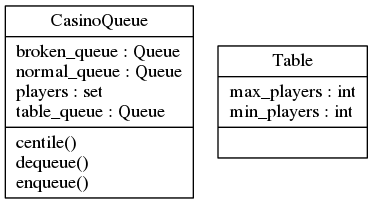
\includegraphics[resolution=130]{figures/diagramme-casino.png}
  \caption{Diagramme de classes du Casino.}
\end{figure}

\begin{figure}
  \centering
  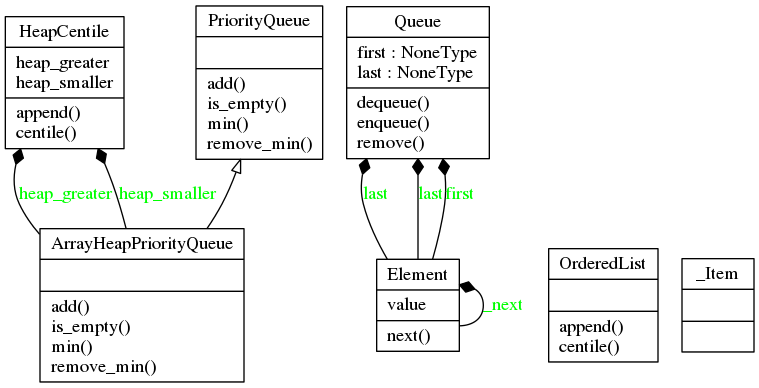
\includegraphics[resolution=130]{figures/diagramme-datastructures.png}
  \caption{Diagramme de classes des structures de données}
\end{figure}

\subsubsection{Classe \textsf{Queue}}
Notre implémentation du Casino est basée sur la classe Queue. La file est
représentée par une liste simplement chainée. Elle respecte l'interface
\textsf{enqueue} \textsf{dequeue} et \textsf{remove}. 

Elle utilise les fonctions magiques de Python pour fournir un iterable, la
longueur, l'élément suivant, l'appartenance et la valeur booléen. C'est une
approche qui facilite l'implémentation et qui favorise une utilisation simple de
la structure de donnée.

\subsubsection{Classe \textsf{CasinoQueue}}
Les instances de la classe CasinoQueue sont des files à 3 priorités. Elles
possèdent les fonctions de base des files : \textsf{enqueue} et
\textsf{dequeue}. Elle possède 3 files chainées de la classe Queue correspondant
à ses trois priorités (table brisée, changement de table et le reste). Les
éléments mis dans les files sont des tuplets de joueur, temps d'entrée dans la
file et, dans le cas de la file pour changement de table, la table désirée.

Lorsque appelée, la fonction dequeue retire, en tout respect de l'énoncé, une
personne de la file ou retourne une exception \textsf{IndexError} si cela est
impossible. \textsf{dequeue} possède un ordre constant lorsque il y a des éléments
dans la queue pour table brisée et a une ordre linéaire par rapport au nombre de
joueur dans la queue pour changement de table dans tous les autres cas.

Chaque appel de la fonction enqueue vérifie que le nom entrée n'est pas un
doublon d'un nom existant déjà dans le casino. Si ce n'est pas le cas, les
paramètres table et broken détermineront à quelle file sera enqueue le joueur.

Il nous aurait été possible d'implémenter la vérification des doublons par une
itération à travers les 3 queues. Pour cause de mauvaise complexité, nous
avons refusé cette option. Il nous aurait été possible de faire un arbre qui
stocke les noms de tout les joueurs qui sont dans le casino et qui font des
recherches en O(log n). Pour cause de flemmardise, nous avons refusé cette
option. Nous avons implémenté \_\_contains\_\_ qui test l'appartenance à un
objet à self.players (un set!)lors de l'entrée d'un nouveau joueur dans le
casino (ajout d'un joueur à la normal\_queue).

\subsubsection{Analyse empirique de \textsf{Queue}}
Tous les tests ont été exécutés sur 500 entrées.

\begin{figure}
\caption{Temps d'exécution de \textsf{enqueue} en fonction du nombre d'entrée.}
\end{figure}
On constate que la file enqueue en temps constant.

\begin{figure}
\caption{Temps d'exécution de \textsf{dequeue} en fonction du nombre d'entrée.}
\end{figure}
On constate que la file dequeue en temps constant.

\begin{figure}
\caption{Temps d'exécution de \textsf{remove} en fonction du nombre d'entrée.}
\end{figure}
Dans ce cas, la file était initialisé à 500 items à chaque opération. On
constate qu'enlever un élément de la liste se fait en temps linéaire sur le
nombre d'éléments.

\section{Calcul du n-ième centile}
Les centils sont calculés avec soit une liste ordonnée \textsf{OrderedList} ou
deux monceaux. L'implantation du monceaux était celle fournit avec dans le cadre
du cours. Les calculateurs étaient interfacés pour fournir une méthode unique
d'ajout \textsf{append}, qui est testé dans ce cas d'analyse.

\subsection{Calcul de centile par une liste ordonnée}
\begin{figure}
\caption{Temps d'exécution de \textsf{append} en fonction du nombre d'entrée.}
\end{figure}
Dans ce cas, la file était initialisé à 500 items à chaque opération. On
constate qu'enlever un élément de la liste se fait en temps linéaire sur le
nombre d'éléments.

\subsection{Calcul de centile par deux monceaux}
\begin{figure}
\caption{Temps d'exécution de \textsf{append} en fonction du nombre d'entrée.}
\end{figure}
Dans ce cas, la file était initialisé à 500 items à chaque opération. On
constate qu'enlever un élément de la liste se fait en temps linéaire sur le
nombre d'éléments.
\end{document}
